
\documentclass{article}
\usepackage[utf8]{inputenc} % Bảng mã UTF-8
\usepackage[english,vietnamese]{babel} % Ngôn ngữ Việt
\usepackage{graphicx}

\title{Báo cáo thực nghiệm với giải thuật di truyền}
\author{Sinh viên thực nghiệm: Nguyễn Trung Hiệp}
\date{\today}

\begin{document}
	\maketitle
	
	\section{Giới thiệu}
	
	Giải thuật Di truyền là một phương pháp tối ưu hóa tự nhiên mạnh mẽ được lấy cảm hứng từ quá trình tiến hóa trong tự nhiên. Thuật toán này đã được áp dụng thành công trong nhiều lĩnh vực từ tối ưu hóa đến học máy và tạo ra sự quan tâm lớn trong cộng đồng nghiên cứu.
	
	Trong báo cáo này, chúng tôi sẽ nêu ý chính và mục tiêu của thí nghiệm sử dụng giải thuật Di truyền, cũng như cách thức thực hiện thí nghiệm và dự kiến kết quả.
	
	\section{Ý chính và Mục tiêu}
	
	\begin{enumerate}
		\item Ý chính:
		- Nghiên cứu và đánh giá hiệu quả của giải thuật Di truyền trong việc tối ưu hóa hàm mục tiêu đa nhiệm.
		\item Mục tiêu:
		\begin{enumerate}
			 \item Thực hiện thí nghiệm để so sánh hiệu suất của giải thuật Di truyền với các phương pháp tối ưu hóa khác trong việc giải quyết các bài toán tối ưu hóa đa nhiệm.
			\item Đánh giá khả năng của giải thuật Di truyền trong việc tìm ra các giải pháp tối ưu đa nhiệm với hiệu suất cao và đồng thời.
		\end{enumerate}
	\end{enumerate}

\section{Phương pháp thực hiện}

\begin{itemize}
	\item Sử dụng ngôn ngữ lập trình Python và thư viện thí nghiệm phổ biến như NumPy, SciPy và scikit-learn.
	\item Thực hiện việc triển khai giải thuật Di truyền và các phương pháp so sánh khác cho các bài toán tối ưu hóa đa nhiệm.
	\item Lập kế hoạch và thực hiện các thí nghiệm với các tập dữ liệu thực tế và các bài toán tối ưu hóa đa nhiệm tiêu biểu.
	\item Đo lường và phân tích kết quả của giải thuật Di truyền so với các phương pháp so sánh khác.
\end{itemize}

\section{Dự kiến kết quả}

\begin{itemize}
	\item Dự kiến rằng giải thuật Di truyền sẽ có hiệu suất tốt trong việc giải quyết các bài toán tối ưu hóa đa nhiệm so với các phương pháp so sánh khác.
	\item Dự kiến rằng giải thuật Di truyền sẽ cho ra các giải pháp tối ưu đa nhiệm với hiệu suất cao và đồng thời trong các bài toán thử nghiệm.
\end{itemize}
\section{Luồng Hoạt Động}

\begin{figure}[h]
	\centering
	\begin{minipage}{0.45\textwidth}
		\centering
		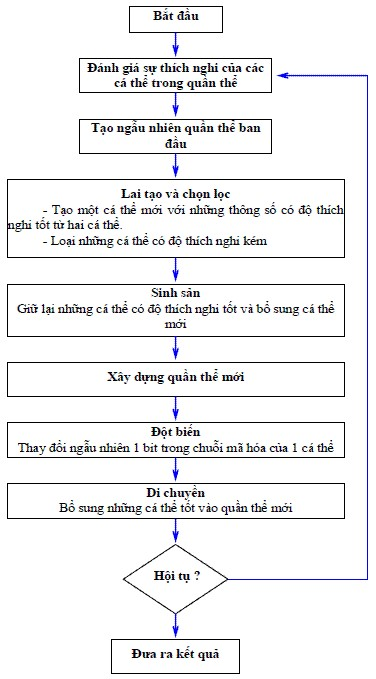
\includegraphics[width=\textwidth]{H:/Đồ án tốt nghiệp/Sơ đồ giải thuật di truyền.jpg}
		\caption{Sơ đồ giải thuật di truyền}
		\label{fig:genetic_algorithm_diagram}
	\end{minipage}\hfill
	\begin{minipage}{0.55\textwidth}
		Luồng hoạt động của giải thuật di truyền có thể được mô tả như sau:
		\begin{enumerate}
			\item \textbf{Khởi tạo quần thể ban đầu}: Bắt đầu với một quần thể ban đầu gồm các cá thể ngẫu nhiên.
			\item \textbf{Đánh giá hiệu suất}: Sử dụng hàm mục tiêu để đánh giá hiệu suất của từng cá thể trong quần thể.
			\item \textbf{Lựa chọn tự nhiên}: Chọn ra các cá thể tốt nhất để tiếp tục vào thế hệ tiếp theo.
			\item \textbf{Lai ghép}: Kết hợp thông tin gen từ hai cá thể cha mẹ để tạo ra các cá thể con mới.
			\item \textbf{Đột biến}: Thực hiện các thay đổi ngẫu nhiên trên gen của các cá thể con để tạo ra sự đa dạng gen mới.
			\item \textbf{Tạo thế hệ tiếp theo}: Tạo ra một thế hệ mới của quần thể bằng cách kết hợp các cá thể cha mẹ, cá thể con mới và các cá thể được chọn từ thế hệ trước đó.
			\item \textbf{Lặp lại}: Lặp lại quá trình trên cho đến khi điều kiện dừng được đạt được, chẳng hạn như số lần lặp cố định hoặc sự hội tụ của giải pháp.
		\end{enumerate}
	\end{minipage}
\end{figure}

\section{Kết luận}
\begin{itemize}

	\item Bằng cách nghiên cứu và thực hiện các thí nghiệm được mô tả, chúng tôi mong đợi sẽ có những nhận thức mới về hiệu quả và khả năng ứng dụng của giải thuật Di truyền trong việc giải quyết các bài toán tối ưu hóa đa nhiệm.
\end{itemize}


\end{document}